\chapter{Organisasi atau Lingkungan Kerja Praktik}

\section{Struktur Organisasi}
PT Radya Anugrah Digital merupakan bagian dari Radya Group. Radya Group terdiri atas Radya Labs Teknologi sebagai perusahaan induk serta beberapa perusahaan yang bergerak di bidang berbeda, yaitu Radya Anugrah Digital, Raditya Alkademi Digital, Radya Acceleration Digital, dan Radya Tosanarka Vidia (Radya Labs 2023). Radya Anugrah Digital bergerak di bidang pengembangan perangkat lunak dan menjadi tempat kami melaksanakan KP. Gambar~\ref{fig:struktur-grup} menunjukkan posisi Radya Anugrah Digital di Radya Group, dengan arsiran untuk tempat kami bekerja.

\begin{figure}[H]
\centering
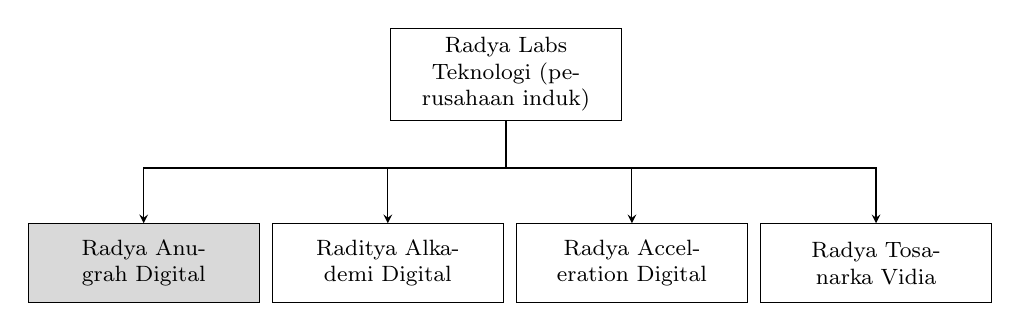
\begin{tikzpicture}[font=\footnotesize,>=stealth,
  box/.style={draw,minimum width=2.9cm,minimum height=1cm,align=center,text width=2.7cm},
  hl/.style={box,fill=black!15}]
\node[box] (induk) at (0,0) {Radya Labs Teknologi (perusahaan induk)};
\node[hl] (rad) at (-4.6,-2.4) {Radya Anugrah Digital};
\node[box] (alk) at (-1.5,-2.4) {Raditya Alkademi Digital};
\node[box] (aks) at (1.6,-2.4) {Radya Acceleration Digital};
\node[box] (tos) at (4.7,-2.4) {Radya Tosanarka Vidia};
\foreach \n in {rad,alk,aks,tos}{\draw[->] (induk.south) -- ++(0,-0.6) -| (\n.north);}
\end{tikzpicture}
\caption{Posisi PT Radya Anugrah Digital dalam Radya Group (diolah dari Radya Labs 2023)}
\label{fig:struktur-grup}
\end{figure}

Di dalam proyek Komatsu ESS, tim dipimpin oleh \textit{Project Manager} yang sekaligus menjadi \textit{mentor} kami. Di bawahnya terdapat tim \textit{developer} dan tim \textit{Quality Assurance} (QA). Gambar~\ref{fig:struktur-tim} menunjukkan struktur tim tersebut, dengan arsiran untuk tim tempat kami bekerja.

\begin{figure}[H]
\centering
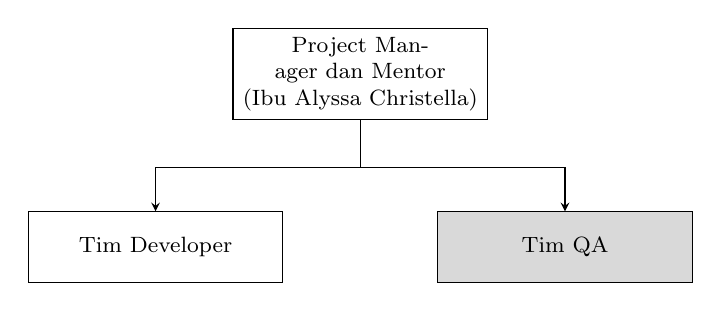
\begin{tikzpicture}[font=\footnotesize,>=stealth,
  box/.style={draw,minimum width=3.2cm,minimum height=0.9cm,align=center,text width=3cm},
  hl/.style={box,fill=black!15}]
\node[box] (pm) at (0,0) {Project Manager dan Mentor\\(Ibu Alyssa Christella)};
\node[box] (dev) at (-2.6,-2.2) {Tim Developer};
\node[hl] (qa) at (2.6,-2.2) {Tim QA};
\foreach \n in {dev,qa}{\draw[->] (pm.south) -- ++(0,-0.6) -| (\n.north);}
\end{tikzpicture}
\caption{Struktur tim proyek Komatsu ESS}
\label{fig:struktur-tim}
\end{figure}

\section{Unit Kerja}

\subsection{Tim Proyek Komatsu ESS}
Kami ditempatkan pada tim proyek Komatsu ESS sebagai \textit{Quality Assurance}. \textit{Project Manager} proyek ini sekaligus \textit{mentor} kami adalah Ibu Alyssa Christella. Selain beliau, tim proyek terdiri atas tim \textit{developer} dan tim QA. Kami bekerja berdua sebagai mahasiswa KP, yaitu Naufarrel Zhafif Abhista dan Zulfaqqar Nayaka Athadiansyah, yang sama-sama berperan sebagai \textit{Quality Assurance}.

\subsection{Lingkup Pekerjaan Tim QA}
Tim QA memastikan aplikasi yang dikembangkan sesuai kebutuhan klien sebelum diserahkan. Caranya dengan menyusun \textit{test script}, menjalankan pengujian, melaporkan \textit{bug} ke \textit{developer}, dan memverifikasi perbaikannya. Pekerjaan kami bagian dari tugas itu, yaitu menguji modul-modul Komatsu ESS yang ditugaskan Ibu Alyssa. Peran kami dirangkum pada Tabel~\ref{tab:peran-kp}.

\begin{table}[H]
\caption{Peran mahasiswa KP pada tim QA proyek Komatsu ESS}
\label{tab:peran-kp}
\centering
\begin{tabularx}{\textwidth}{|p{4.2cm}|p{2.6cm}|X|}
\hline
\textbf{Nama} & \textbf{Peran} & \textbf{Tanggung Jawab} \\
\hline
Naufarrel Zhafif Abhista (13523149) & \textit{Quality Assurance} & Menyusun \textit{test script}, menguji, dan melaporkan \textit{bug} pada modul yang ditugaskan; \textit{integration testing} dan regresi bersama \\
\hline
Zulfaqqar Nayaka Athadiansyah (13523094) & \textit{Quality Assurance} & Menyusun \textit{test script}, menguji, dan melaporkan \textit{bug} pada modul yang ditugaskan; \textit{integration testing} dan regresi bersama \\
\hline
\end{tabularx}
\end{table}

\section{Deskripsi Pekerjaan}
Pekerjaan kami terbagi menjadi enam tahap yang berurutan dan sedikit tumpang tindih, seperti pada Tabel~\ref{tab:tahap-pekerjaan}. Pelaporan \textit{bug} dilakukan pada setiap tahap pengujian. Setiap tahap kami jelaskan di Bab III.

\begin{table}[H]
\caption{Tahapan pekerjaan}
\label{tab:tahap-pekerjaan}
\centering
\begin{tabularx}{\textwidth}{|c|p{3.4cm}|X|}
\hline
\textbf{No.} & \textbf{Tahap} & \textbf{Kegiatan} \\
\hline
1 & Orientasi & Mempelajari aplikasi, alur bisnis, alat kerja, dan prosedur tim \\
\hline
2 & Penyusunan draf \textit{test script} & Menganalisis \textit{requirement} fitur dan menyusun \textit{test script} tiap modul \\
\hline
3 & \textit{Module testing} & Menjalankan \textit{test script} pada masing-masing modul dan melaporkan \textit{bug} \\
\hline
4 & \textit{Integration testing} & Menguji alur yang melibatkan lebih dari satu modul \\
\hline
5 & \textit{Regression testing} & Menjalankan ulang pengujian untuk memverifikasi perbaikan \\
\hline
6 & Dokumentasi & Merangkum hasil pengujian dan menyusun laporan KP \\
\hline
\end{tabularx}
\end{table}

\section{Jadwal Kerja}
KP berlangsung 13 minggu, dari 22 Juni sampai 22 September 2026. Tabel~\ref{tab:jadwal-kerja} menunjukkan gambaran jadwalnya, dan kegiatan harian kami catat di \textit{Log Activity} pada Lampiran B. Jadwal ini mengikuti rencana di TOR (Lampiran A).

\begin{table}[H]
\caption{Gambaran jadwal kegiatan selama KP}
\label{tab:jadwal-kerja}
\centering
\begin{tabularx}{\textwidth}{|p{5cm}|c|X|}
\hline
\textbf{Tahap} & \textbf{Minggu} & \textbf{Keterangan} \\
\hline
Orientasi & 1--2 & Pengenalan lingkungan kerja dan aplikasi \\
\hline
Penyusunan draf \textit{test script} & 2--5 & \textit{Test script} per modul \\
\hline
\textit{Module testing} & 5--9 & Pengujian modul yang ditugaskan \\
\hline
\textit{Integration testing} & 8--11 & Pengujian alur lintas modul \\
\hline
\textit{Regression testing} & 11--12 & Verifikasi perbaikan dan pengujian ulang \\
\hline
Dokumentasi dan laporan KP & 12--13 & Penyusunan laporan dan penilaian \\
\hline
\end{tabularx}
\end{table}
